\documentclass[letterpaper,12pt]{article}
\usepackage{array}
\usepackage{threeparttable}
\usepackage{geometry}
\geometry{letterpaper,tmargin=1in,bmargin=1in,lmargin=1.25in,rmargin=1.25in}
\usepackage{fancyhdr,lastpage}
\pagestyle{fancy}
\lhead{}
\chead{}
\rhead{}
\lfoot{}
\cfoot{}
\rfoot{\footnotesize\textsl{Page \thepage\ of \pageref{LastPage}}}
\renewcommand\headrulewidth{0pt}
\renewcommand\footrulewidth{0pt}
\usepackage[format=hang,font=normalsize,labelfont=bf]{caption}
\usepackage{listings}
\lstset{frame=single,
  language=Python,
  showstringspaces=false,
  columns=flexible,
  basicstyle={\small\ttfamily},
  numbers=none,
  breaklines=true,
  breakatwhitespace=true
  tabsize=3
}
\usepackage{amsmath}
\usepackage{amssymb}
\usepackage{amsthm}
\usepackage{harvard}
\usepackage{setspace}
\usepackage{float,color}
\usepackage[pdftex]{graphicx}
\usepackage{hyperref}
\hypersetup{colorlinks,linkcolor=red,urlcolor=blue}
\theoremstyle{definition}
\newtheorem{theorem}{Theorem}
\newtheorem{acknowledgement}[theorem]{Acknowledgement}
\newtheorem{algorithm}[theorem]{Algorithm}
\newtheorem{axiom}[theorem]{Axiom}
\newtheorem{case}[theorem]{Case}
\newtheorem{claim}[theorem]{Claim}
\newtheorem{conclusion}[theorem]{Conclusion}
\newtheorem{condition}[theorem]{Condition}
\newtheorem{conjecture}[theorem]{Conjecture}
\newtheorem{corollary}[theorem]{Corollary}
\newtheorem{criterion}[theorem]{Criterion}
\newtheorem{definition}[theorem]{Definition}
\newtheorem{derivation}{Derivation} % Number derivations on their own
\newtheorem{example}[theorem]{Example}
\newtheorem{exercise}[theorem]{Exercise}
\newtheorem{lemma}[theorem]{Lemma}
\newtheorem{notation}[theorem]{Notation}
\newtheorem{problem}[theorem]{Problem}
\newtheorem{proposition}{Proposition} % Number propositions on their own
\newtheorem{remark}[theorem]{Remark}
\newtheorem{solution}[theorem]{Solution}
\newtheorem{summary}[theorem]{Summary}
%\numberwithin{equation}{section}
\bibliographystyle{aer}
\newcommand\ve{\varepsilon}
\newcommand\boldline{\arrayrulewidth{1pt}\hline}
\begin{document}

% ----------------------------------------------------------------------
\begin{flushleft}
  \textbf{\large{Problem Set \#3}} \\
  MACS 30100, Dr. Evans \\
  Chih-Yu Chiang \\
  Python Version: 3.5.2
\end{flushleft}
\vspace{5mm}
\noindent\textbf{Problem 1} \\
\\
The minimization processes in the 4 estimations in (b) to (e) all succeeded.
For acquiring converged results from the algorithms, the estimation settings are as follow: \\
(b). error simple mode = False; minimization method = L-BFGS-B. \\
(c). error simple mode = False; minimization method = TNC. \\
(d). error simple mode = True; minimization method = L-BFGS-B. \\
(e). error simple mode = True; minimization method = TNC. \\

\noindent\textbf{Part (a). histogram} \\
\\
A histogram of annual incomes of students who graduated in 2018, 2019, and 2020 from the University of Chicago M.A. Program in Computational Social Science. \\
\\
\begin{figure}[htb]\centering\captionsetup{width=6.0in}
  \caption{\textbf{}}
  \fbox{\resizebox{4.0in}{3.0in}{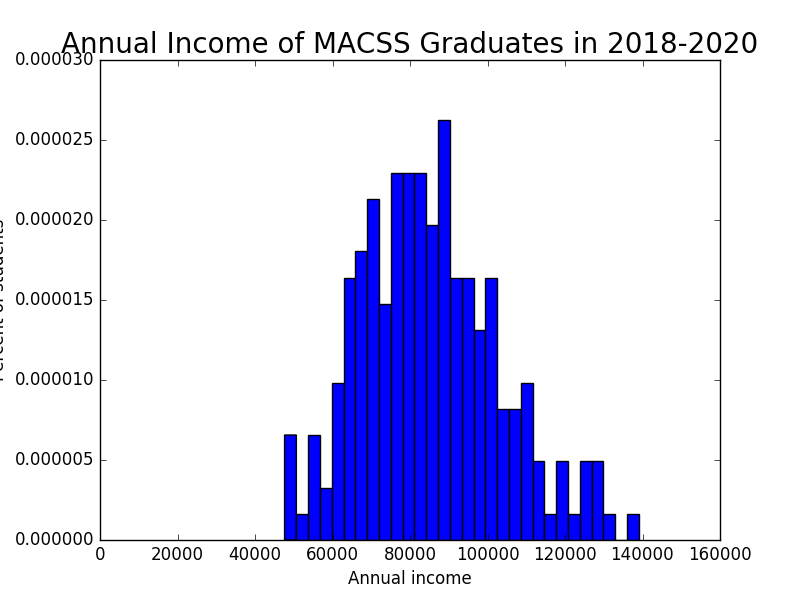
\includegraphics{1a.png}}}
\end{figure} \\

\clearpage

% ----------------------------------------------------------------------
\noindent\textbf{Part (b). One step GMM with mean and std} \\
\\
One step GMM is estimated with mean and standard deviation as moments and identity weighting matrix. The initial guess of $\mu$ is 11 and $\sigma$ is 0.2.\\
The resulted criterion value is 8.97474397e-15. The estimated parameters are as follow:
\[\mu_{GMM1}= 11.3317738625\]
\[\sigma_{GMM1}= 0.209209064254\]

\begin{center}
\begin{tabular}{ c|c|c }
 moments & mean & var \\
 \hline
 data & 85276.82360625808 & 325358364.0497777 \\
 model & 85276.8309999 & 325358351.628 \\
 data - model & -0.00739366149355 & 12.4213916063
\end{tabular}
\end{center}
\\

A lognormal pdf with estimated parameters is plotted. \\

\begin{figure}[htb]\centering\captionsetup{width=6.0in}
  \caption{\textbf{}}
  \fbox{\resizebox{4.0in}{3.0in}{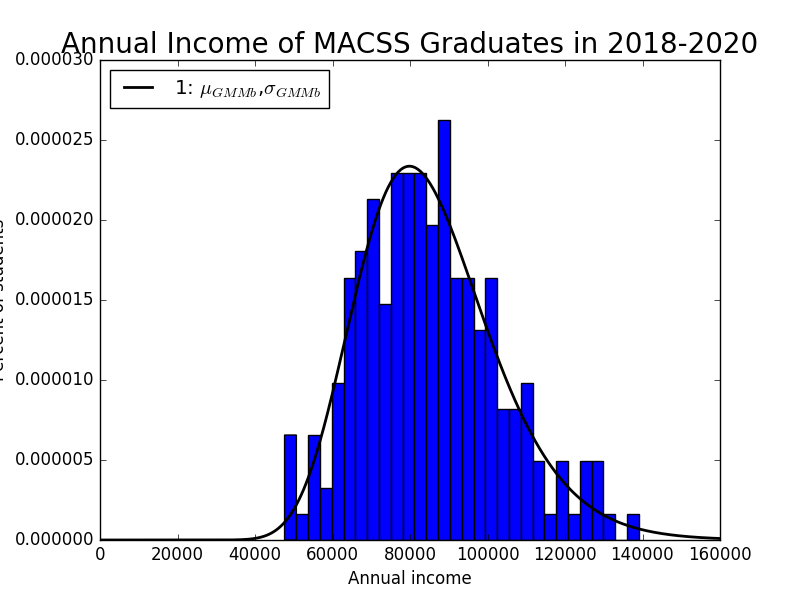
\includegraphics{1b.png}}}
\end{figure} \\

\clearpage

% ----------------------------------------------------------------------
\noindent\textbf{Part (c). Two step GMM with mean and std} \\
\\
Two step GMM is estimated with mean and standard deviation as moments and weighting matrix derived from (b). The initial guess of $\mu$ and $\sigma$ is the estimated results from (b). \\
The resulted criterion value is 6.98194849. The estimated parameters are as follow:
\[\mu_{GMM2}= 11.3317737968\]
\[\sigma_{GMM2}= 0.209209082101\]

\begin{center}
\begin{tabular}{ c|c|c }
 moments & mean & var \\
 \hline
 data & 85276.82360625808 & 325358364.0497777 \\
 model & 85276.8257185 & 325358368.061 \\
 data - model & -0.00211221084464 & -4.01102161407
\end{tabular}
\end{center}
\\

Lognormal pdfs with estimated parameters in previous and this questions are plotted. \\

\begin{figure}[htb]\centering\captionsetup{width=6.0in}
  \caption{\textbf{}}
  \fbox{\resizebox{4.0in}{3.0in}{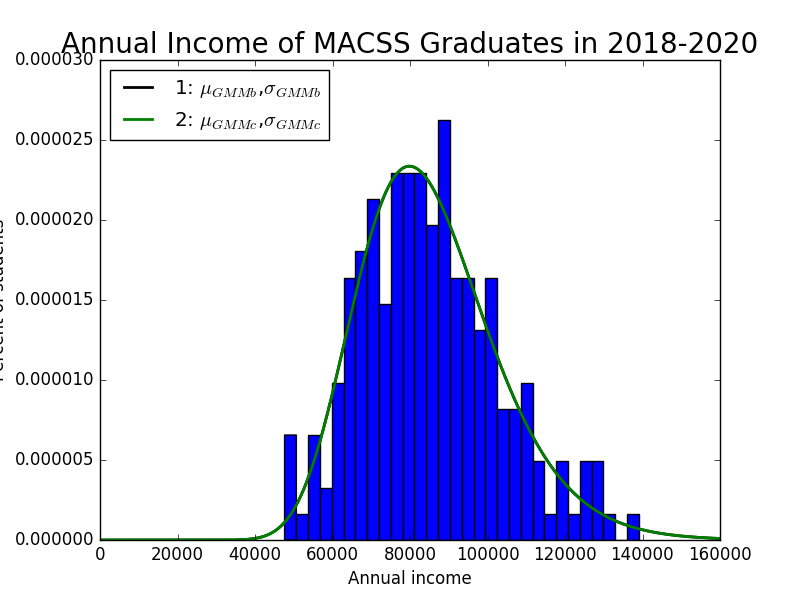
\includegraphics{1c.png}}}
\end{figure} \\

\clearpage

% ----------------------------------------------------------------------

\noindent\textbf{Part (d). One step GMM with three proportion moments} \\
\\
One step GMM is estimated with percent of individuals who earn less than \$75,000,  between \$75,000 and \$100,000, and more than \$100,000 as moments and identity weighting matrix. The initial guess of $\mu$ is 11 and $\sigma$ is 0.2. \\
The resulted criterion value is 6.36574754e-15. The estimated parameters are as follow:
\[\mu_{GMM1_3}= 11.3356813687\]
\[\sigma_{GMM1_3}= 0.210598464642\]

\begin{center}
\begin{tabular}{ c|c|c|c }
 moments & less than 75,000 & 75,000-100,000 & more than 100,000 \\
 \hline
 data & 0.3 & 0.5 & 0.2 \\
 model & 0.2999999448933023 & 0.4999999974649346 & 0.2000000576417631 \\
 data - model & 5.510669770503185e-08 & 2.535065379838386e-09 & -5.7641763084870234e-08
\end{tabular}
\end{center}
\\

A lognormal pdf with estimated parameters is plotted. \\

\begin{figure}[htb]\centering\captionsetup{width=6.0in}
  \caption{\textbf{}}
  \fbox{\resizebox{4.0in}{3.0in}{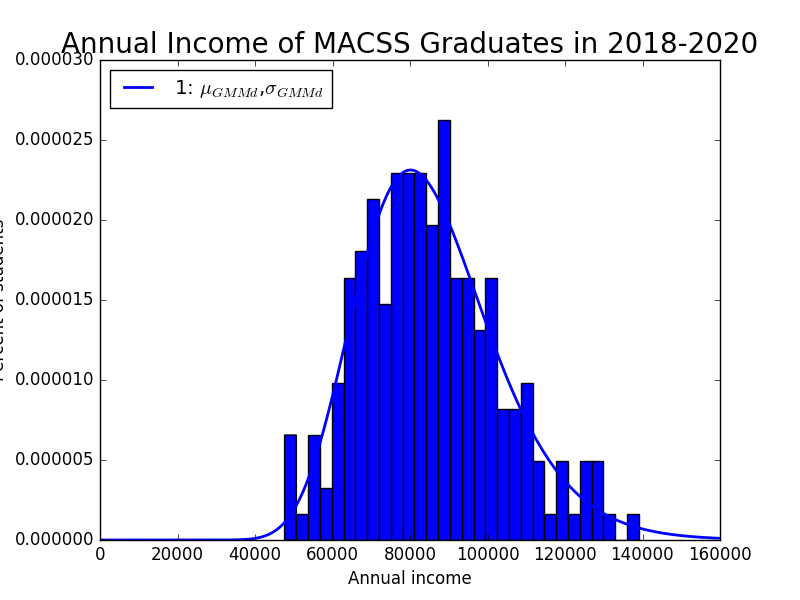
\includegraphics{1d.png}}}
\end{figure} \\
\\
\clearpage

% ----------------------------------------------------------------------
\noindent\textbf{Part (e). Two step GMM with three proportion moments} \\
\\
Two step GMM is estimated with percent of individuals who earn less than \$75,000,  between \$75,000 and \$100,000, and more than \$100,000 as moments and weighting matrix derived from (d). The initial guess of $\mu$ and $\sigma$ is the estimated results from (d). \\
The resulted criterion value is 2.6828065. The estimated parameters are as follow:
\[\mu_{GMM2_3}= 11.335681335\]
\[\sigma_{GMM2_3}= 0.210598464603\]

\begin{center}
\begin{tabular}{ c|c|c|c }
 moments & less than 75,000 & 75,000-100,000 & more than 100,000 \\
 \hline
 data & 0.3 & 0.5 & 0.2 \\
 model & 0.3000000005650838 & 0.4999999866894511 & 0.20000001274546508 \\
 data - model & -5.650838130755176e-10 & 1.3310548885314688e-08 & -1.274546507223917e-08
\end{tabular}
\end{center}
\\

Lognormal pdfs with estimated parameters in previous and this questions are plotted. \\

\begin{figure}[htb]\centering\captionsetup{width=6.0in}
  \caption{\textbf{}}
  \fbox{\resizebox{4.0in}{3.0in}{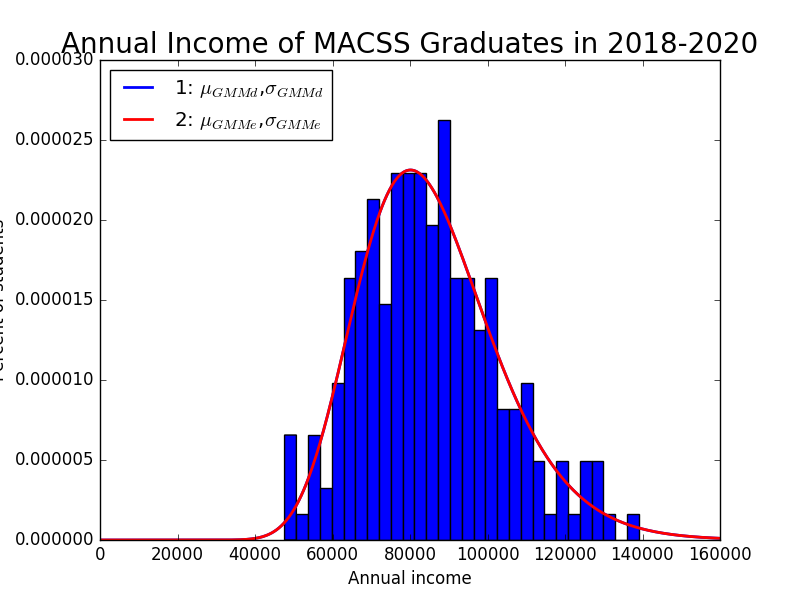
\includegraphics{1e.png}}}
\end{figure} \\
\\
\\
\clearpage

% ----------------------------------------------------------------------
\noindent\textbf{Part (f). Estimation comparison} \\
\\
From the following reasoning, I deem the estimation from (e) fits the data best. \\
The pdf from (b) and (c) estimations are visually indistinguishable in the plot. Though, comparing the difference of data moment and model moment of these two estimations, we can still find that the two-step estimation in (c) provides a slightly better result than (b), while the difference of data moment and model moment in (c) is generally smaller than (b). \\
Similarly, the pdf from (d) and (e) estimations are also visually indistinguishable in the plot. Though, comparing the difference of data moment and model moment of these two estimations, we can still find that the two-step estimation in (e) provides a slightly better result than (d), while the difference of data moment and model moment in (e) is generally smaller than (d). \\
Visually comparing estimations from (c) and (e), one can tell that (c) covers more data in the middle range while (e) more in the tails. Based on the real data distribution, I would say estimation from (e) is slightly better than (c) since it covers more and has better description around the range 100,000 to 140,000, where the two pdfs generally can not describe the real data very well and I believe should be better addressed.

\begin{figure}[htb]\centering\captionsetup{width=6.0in}
  \caption{\textbf{}}
  \fbox{\resizebox{4.0in}{3.0in}{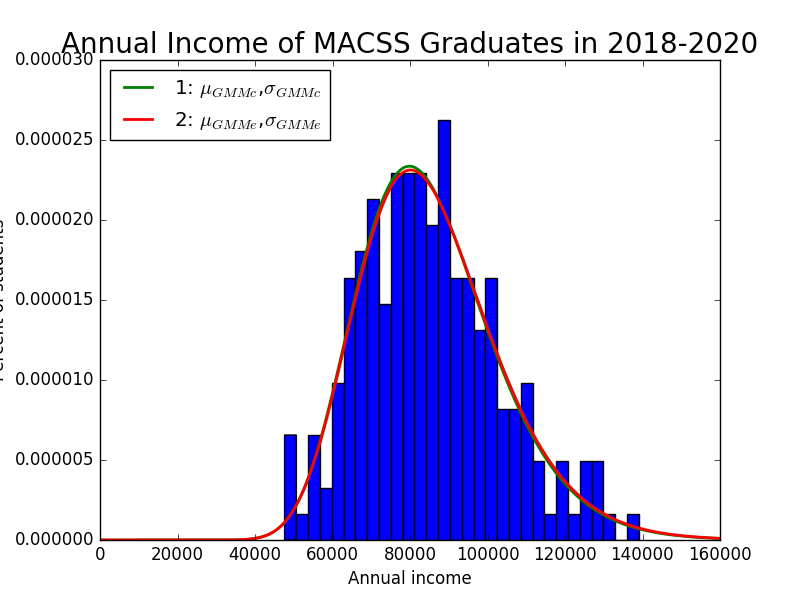
\includegraphics{1c+1e.png}}}
\end{figure} \\
\\
\\
\\
\clearpage

% ----------------------------------------------------------------------
\noindent\textbf{Note:}\\
The above estimations in (c) and (e) are based on the parameters estimated in (b) and (d) respectively as initial guess. \\
I also tried applying $\mu = 11$ and $\sigma = 0.2$ as the initial guess in (c) and (e); this yielded worse fits as the images shown below and thus are not considered in the answers of (c), (e), and (f). The code applying constant initial guess values to (c) and (e) can be accessed in "PS3\_with\_constant\_initial\_guess.py". The corresponding estimation results and criterion values are also computed when running the mentioned Python file.

\begin{figure}[htb]\centering\captionsetup{width=6.0in}
  \caption{\textbf{}}
  \fbox{\resizebox{3.5in}{2.5in}{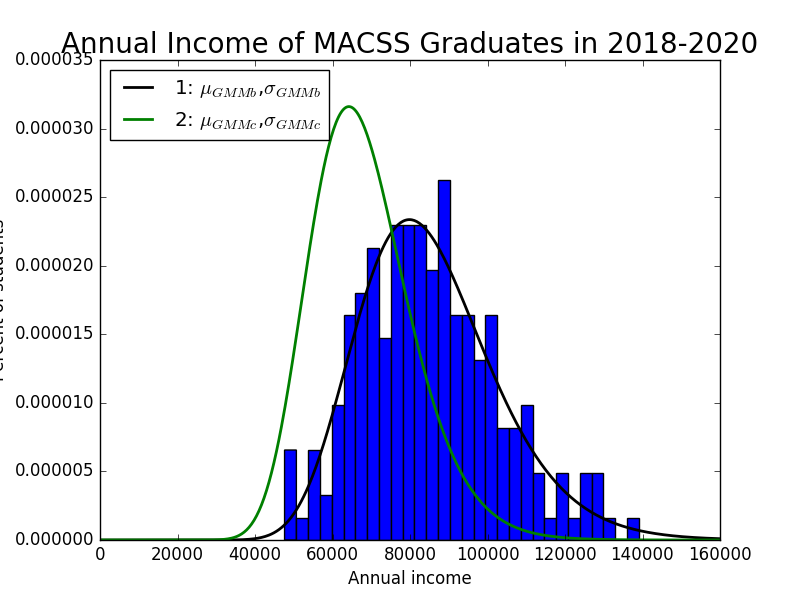
\includegraphics{1c_constant.png}}}
\end{figure} \\

\begin{figure}[htb]\centering\captionsetup{width=6.0in}
  \caption{\textbf{}}
  \fbox{\resizebox{3.5in}{2.5in}{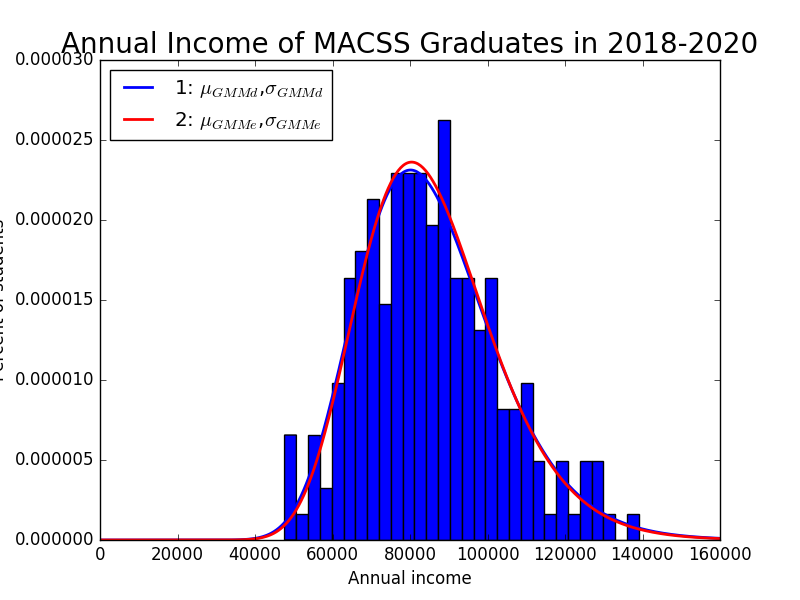
\includegraphics{1e_constant.png}}}
\end{figure} \\
\\
\\
\clearpage

% ----------------------------------------------------------------------
\noindent\textbf{Problem 2} \\
\noindent\textbf{Part (a). Linear regression and GMM} \\
\\
GMM is estimated with real and estimated sick data as moments and identity weighting matrix. The initial guesses for $\beta_0$, $\beta_1$, $\beta_2$, $\beta_3$ are 0, 0, 0, 1.\\
The resulted criterion value is 0.0018212898429. The estimated parameters are as follow: \\
\[\beta_{0, GMM}= 0.251644806982\]
\[\beta_{1, GMM}= 0.0129334340231\]
\[\beta_{2, GMM}= 0.400501320535\]
\[\beta_{3, GMM}= -0.00999168732927\]
\\

\end{document}
